
\DeclareRobustCommand{\dlo}[1]{}
\DeclareRobustCommand{\wen}[1]{#1}
\DeclareRobustCommand{\old}[1]{}
\DeclareRobustCommand{\new}[1]{#1}



\title{Accelerated signal-and-noise orthogonalization}
\renewcommand{\thefootnote}{\fnsymbol{footnote}}
\author{Guangtan Huang, Dong Zhang, Wei Chen, and Yangkang Chen}
%\author{Guangtan Huang, Dong Zhang, Wei Chen, and Yangkang Chen
%\thanks{G. Huang and Y. Chen are with Key Laboratory of Geoscience Big Data and Deep Resource of Zhejiang Province, School of Earth Sciences, Zhejiang University, Hangzhou 310027, China.}
%\thanks{D. Zhang is Department of Imaging Physics, Delft University of Technology, Lorentzweg 1, 2628 CJ, Delft, The Netherlands.}
%\thanks{W. Chen is with Key Laboratory of Exploration Technology for Oil and Gas Resources of Ministry of Education, Yangtze University, Wuhan 430100, China.}
%\thanks{This work was supported in part by the Starting Fund from Zhejiang University, the National Natural Science Foundation of China under Grant 41804140, and the Open Fund of Key Laboratory of Exploration Technologies for Oil and Gas Resources (Yangtze University), Ministry of Education, under Grant PI2018-02. (Corresponding authors: Wei Chen)}}
\maketitle

\begin{abstract}
The local signal-to-noise orthogonalization algorithm has been widely used in the community of seismic processing and imaging. It helps orthogonalize the signal and noise components in an elegant way so that the noise does not contain the signal leakage in seismic denoising. %a denoising application.  or the wave components are better separated in a wavefield propagation problem. 
The traditional local signal-to-noise orthogonalization is based on solving a highly under-determined ill-posed inverse problem with local smoothness constraint. Due to the inversion nature, the local orthogonalization method requires a large number of iterations, and thus is computationally demanding in large-scale applications. Here, we proposed a much accelerated signal-and-noise orthogonalization method, where we design an efficient way for calculating the orthogonalization weight. When new samples are involved in the calculation, we calculate the orthogonalization weight of the new samples by connecting them with the calculated weights of previous samples. The orthogonalization weight needs to be smoothed and scaled after all samples have been processed to make the resulted orthogonalization weight smooth across the seismic data and match the amplitude level of the initially suppressed noise. In this way, we avoid iterations when calculating the orthogonalization weight. We apply the proposed method to several synthetic and field data examples, have a benchmark comparison with state-of-the-art algorithms, and demonstrate its much accelerated efficiency compared with the traditional local signal-and-noise orthogonalization.
\end{abstract}

%\begin{keywords}
%Denoising, local orthogonalization, seismic data processing
%\end{keywords}

\section{Introduction}
The seismic data profile is composed of different components, e.g., useful signals and unwanted noise. To enhance the useful components while rejecting those unwanted components has been an exclusively studied research topic \cite{canales1984,yangkang20141,yanan2014,yangkang20142,curveletieee2016,mostafa2016geo,weilin2016dmssa,xue2017full,shaohuan2018ieee,wang2019hankel,yangkang2019nc,wang2019efficient,omar2020geo1,wanghang2021geo}. Generally, such components play different roles depending on the purpose. In conventional processing, components other than the primary reflected waves are often considered as noise. However, with the development of exploration technology, many components that are considered noise have gradually been accepted and considered to be very useful. For instance, multiple waves, which have long been regarded as noise in conventional processing, are an important part of the full wavefield imaging and inversion \cite{verschuur2011}.  Such a relationship is also reflected in the diffracted wave to the diffraction imaging \cite{fomel2007}. Moreover, the interfering ambient noise can also be considered as signals when it comes to passive source seismic survey \cite{de2011ambient}. Thus, noise and signals themselves are not absolute concepts, which all depend on whether the signal component is needed for the undergoing work. Here, the signal is defined as those desired components in the seismic profiles, while noise is exploited to refer to the rest unwanted components. Therefore, how to separate the required and non-required components in the signal according to certain characteristics has an important role in the seismic data processing.

Chen and Fomel (2015) \cite{yangkang2015ortho} first proposed a secondary processing step, which is so-called the local signal-and-noise orthogonalization, to optimize the separation of signal and noise components after initial processing.  Such an algorithm effectively solve the signal leakage problem, which is a commonly existing problem in denoising processing. Local signal-and-noise orthogonalization makes use of the local orthogonality of signal and noise to separate the two without leakage. However, traditional methods always cause more or less signal leakage due to wrong parameter selection or insufficient denoising assumptions. Instead of using such a long name, here we use the local orthogonalization method to indicate this algorithm throughout this article for simplicity. The local orthogonalization method can retrieve the lost signal energy from the noise eliminated by a traditional denoising algorithm by using an element-wise weighting operator. Such an operator can be obtained by solving an inverse problem, where the model is constrained by a smoothing operator. 

The local orthogonalization method has first demonstrated the performance via random noise attenuation \cite{yangkang2015ortho}. Although there are many methods for random noise suppression, the signal leakage problem still exists in these traditional methods. The local orthogonalization method effectively improves the denoising performance, and avoids the leakage of the effective signal as much as possible, and lays the foundation for subsequent imaging and inversion. Then, the algorithm has been widely exploited in some other seismic denoising processing, including ground roll noise removal, deblending, and demultiple, etc. Chen et al. (2015) \cite{yangkang2015orthogroll} then applied this method to help to suppress the ground roll noise. This approach is also based on the low-pass filtering based method to remove the ground roll noise, and then retrieve those reflection components that should not be suppressed from the removed noise.  In a similar way, Chen (2015) \cite{yangkang2015dbortho} introduced the algorithm into the iterative simultaneous-source separation framework \cite{yangkang20142,shaohuan2019} to improve the deblending effect. Introducing the local orthogonalization method in each iteration greatly improves the deblending performance and accelerates the convergency. \cite{zhangdong2019ortho} combined the algorithm with the surface-related multiple elimination (SRME) to retrieve the leaked multiples energy in the initially demultipled data, which effectively separate the primaries and multiples. \cite{zhangdong2020geo} further used the local orthogonalization method to suppress internel multiples from full-wavefield migrated images.

In addition to noise removal, the local orthogonalization method has also been widely used in wavefield decomposition. By compensating the amplitude leakage in each separated wave component, Sripanich et al. (2017) \cite{sripanich2017elastic} applied this method to better decompose the elastic wave modes in heterogeneous anisotropic media. Huang et al. (2018) \cite{weilin2018} better decomposed a microseismic trace via introducing the local orthogonalization method into a mathematical morphology algorithm. The improved algorithm decomposed the microseismic trace into quasi-orthogonal components, which can be exploited for weak microseismic signal detection.  Jeong et al. (2019) \cite{jeong2019enhanced} applied this method to the P- and S-components separation of elastic wave forward modeling, and further applied it to the multi-parameter full-waveform inversion (FWI). The inversion results demonstrate that the local orthogonalization method can not only decrease the residual energy or crosstalk caused by using conventional methods, but also accelerate the convergency of multi-parameter FWI and reduce likelihood of being trapped into local minima. Qu et al. (2020) \cite{qu2020robust} applied the local orthogonalization method to tackle the AVO effect in the joint migration inversion (JMI).

Due to the ill-posedness of the inverse problem, the objective function itself is also a function of the target parameters, thus a large number of iterations are required for solving the inverse problem. Similarly, the local orthogonalization method also requires a large number of iterations, and is computationally demanding in large-scale applications. Thus, the computational efficiency is an important bottleneck that limits the large-scale application of the local orthogonalization method in industrial use.  In this paper, to improve computing efficiency, we proposed a much accelerated signal-and-noise orthogonalization method, where we design an efficient way of calculating the orthogonalization weight. When new samples are involved in the calculation, we connect the orthogonalization weights of the new samples with the calculated weight of the previous samples to calculate the orthogonalization weights of the new samples. After processing all samples, the orthogonalization weights need to be smoothed and scaled so that the obtained orthogonalization weights are smoothed in the seismic data and matched with the amplitude level of the initial suppression noise. In this way, iteration is avoided when calculating the orthogonalization weights.

This paper is organized as follows. Firstly, we briefly review the theory of the conventional local signal-and-noise orthogonalization algorithm.  Then, the formula of the non-stationary triangle smoother and the iterative optimization method of adaptively obtaining a smooth radius map are introduced in detail. Next, the performance of the proposed method is proved by a set of representative examples. Finally, we draw some key conclusions.

\begin{figure}[htb!]
\centering
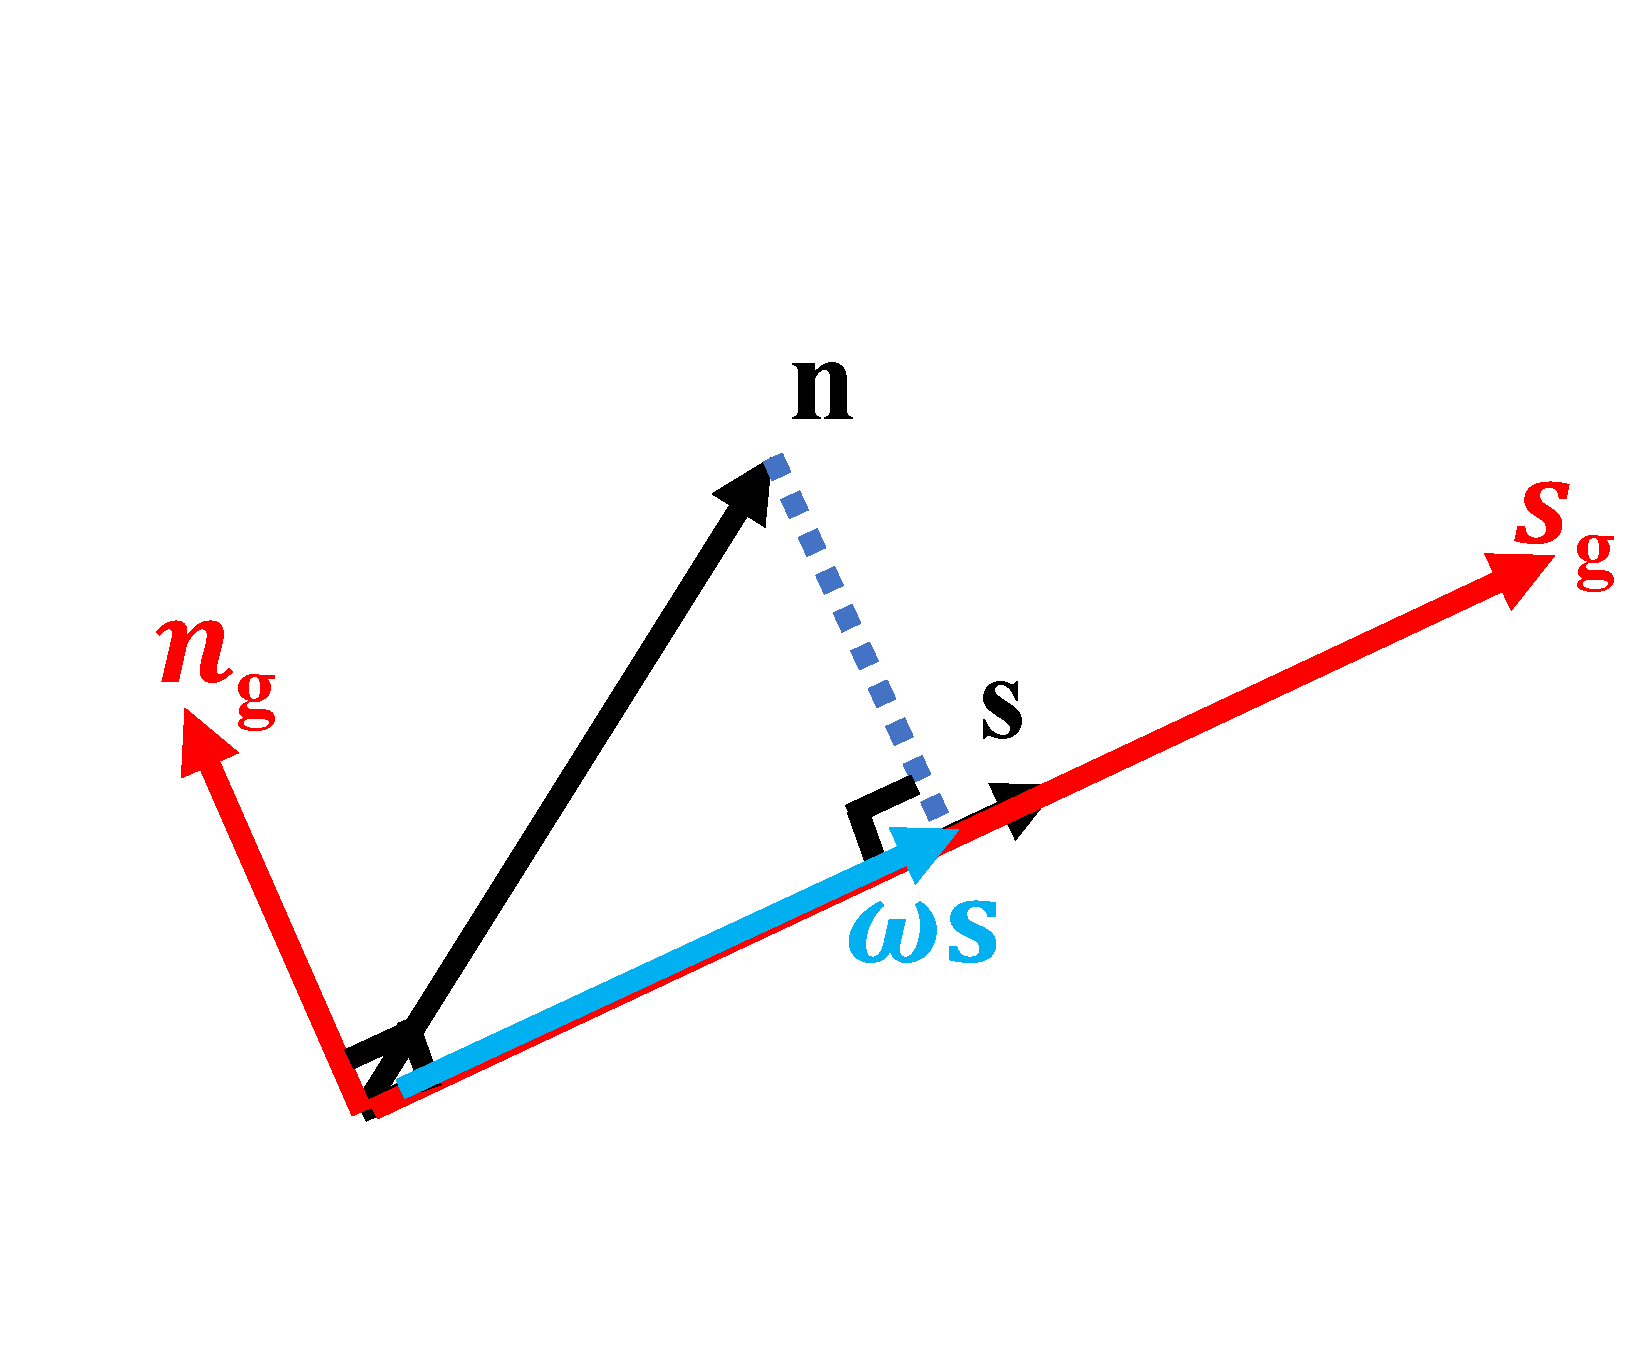
\includegraphics[width=0.45\textwidth]{Fig/demo_vec2}
\caption{Demonstration of the Gram-Schmidt orthogonalization.}
\label{fig:demo_vec2}
\end{figure}

\begin{figure}[htb!]
\centering
\subfloat[]{\includegraphics[width=0.31\columnwidth]{complex/Fig/c}
   \label{fig:c}}
   \subfloat[]{\includegraphics[width=0.31\columnwidth]{complex/Fig/n}
   \label{fig:n}}
\subfloat[]{\includegraphics[width=0.31\columnwidth]{complex/Fig/cn}
   \label{fig:cn}}\\
   \subfloat[]{\includegraphics[width=0.31\columnwidth]{complex/Fig/cfx}
   \label{fig:cfx}}
\subfloat[]{\includegraphics[width=0.31\columnwidth]{complex/Fig/cfx2}
   \label{fig:cfx2}}
   \subfloat[]{\includegraphics[width=0.31\columnwidth]{complex/Fig/cfx22}
   \label{fig:cfx22}}\\  
   \subfloat[]{\includegraphics[width=0.31\columnwidth]{complex/Fig/cdifffx}
   \label{fig:cdifffx}}
\subfloat[]{\includegraphics[width=0.31\columnwidth]{complex/Fig/cdifffx2}
   \label{fig:cdifffx2}}
   \subfloat[]{\includegraphics[width=0.31\columnwidth]{complex/Fig/cdifffx22}
   \label{fig:cdifffx22}}
\caption{Comparison of using the local-orthogonalization-based random noise attenuation approach for denoising test before and after. (a) Clean section. (b) Random noise section. (c) Noisy section (S/N=-0.75 dB). (d) Denoised result using $f$-$x$ deconvolution (S/N=9.21 dB). (e) Denoised result using the traditional orthogonalization method (S/N=10.99 dB). (f) Denoised result using the proposed method (S/N=10.40 dB). (g) Noise section using $f$-$x$ deconvolution. (h) Noise section using traditional orthogonalization method. (i) Noise section using the proposed method.}
\label{fig:c,n,cn,cfx,cfx2,cfx22,cdifffx,cdifffx2,cdifffx22}
\end{figure}

\begin{figure}[htb!]
\centering
\subfloat[]{\includegraphics[width=0.31\columnwidth]{complex/Fig/csimi-difffx}
   \label{fig:csimi-difffx}}
   \subfloat[]{\includegraphics[width=0.31\columnwidth]{complex/Fig/csimi-difffx2}
   \label{fig:csimi-difffx2}}
\subfloat[]{\includegraphics[width=0.31\columnwidth]{complex/Fig/csimi-difffx22}
   \label{fig:csimi-difffx22}}
\caption{(a) Local similarity map using FX method. (b) Local similarity using the traditional orthogonalization method. (c) Local similarity using the proposed accelerated orthogonalization method.}
\label{fig:csimi-difffx,csimi-difffx2,csimi-difffx22}
\end{figure}


\section{Theory}
\subsection{Local signal-and-noise orthogonalization}
Given an input noisy seismic data $\mathbf{d}$, the signal and noise components after applying a normal denoising operator $\mathbf{P}$ can be expressed as:
\begin{align}
\label{eq:sn}
\mathbf{s} &= \mathbf{Pd}\\
\label{eq:snn}
\mathbf{n} &= \mathbf{d} -  \mathbf{Pd},
\end{align}
where $\mathbf{s}$ and $\mathbf{n}$ denote the initial signal and noise components after the initial denoising. 

Due to inappropriate parameter selection or inadequacy of denoising assumptions \cite{yangkang2015ortho},  there will be still signal leakage in the noise component $\mathbf{n}$. The local signal-and-noise orthogonalization method was developed by \cite{yangkang2015ortho} to solve the signal leakage problem. The principle of the local signal-and-noise orthogonalization is to apply a weighting operator to retrieve the leaked signal component:
\begin{align}
\label{eq:sn1}
\hat{\mathbf{s}} &= \mathbf{s} + \tilde{\mathbf{s}},\\
\hat{\mathbf{n}} &= \mathbf{n} -  \tilde{\mathbf{s}},
\end{align}
where $\tilde{\mathbf{s}}$ denotes the leaked signal. The weight operator is expressed as a diagonal matrix composed of a weighting vector. The weighting vector can be obtained by extending the Gram-Schmidt orthogonalization \cite{gram} to a local version. An illustrative Fig. about the Gram-Schmidt orthogonalization is plotted in Fig. \ref{fig:demo_vec2}.  The vectors $\mathbf{s}$ and $\mathbf{n}$ can be orthogonalized by adding a scaled signal component $\mathbf{s}$ to the original signal component and subtracting the scale signal component from the noise component $\mathbf{n}$:
\begin{align}
\label{eq:sn2}
\hat{\mathbf{s}} &= \mathbf{s} + w\mathbf{s},\\
\label{eq:snn2}
\hat{\mathbf{n}} &= \mathbf{n} - w\mathbf{s},
\end{align}
where $\omega$ is a scalar denoting the orthogonalization weight. According to the principle of Gram-Schmidt orthogonalization, it is easy to derive that 
\begin{align}
\label{eq:sn3}
\omega=\frac{\mathbf{s}^T\mathbf{n}}{\mathbf{s}^T\mathbf{s}}.
\end{align}
In contrast to the local orthogonalization, we refer the orthogonalization weight in equation \ref{eq:sn3} as the global orthogonalization weight. The local orthogonalization weight indicates calculating the weight in a local way. The easiest way to define the local orthogonalization weight based on equation \ref{eq:sn3} is as follows:
\begin{align}
\label{eq:low}
w(x_1,x_2,x_3)=\frac{s(x_1,x_2,x_3)n(x_1,x_2,x_3)}{s(x_1,x_2,x_3)s(x_1,x_2,x_3)}=\frac{n(x_1,x_2,x_3)}{s(x_1,x_2,x_3)},
\end{align}
where $x_1,x_2,x_3$ denote the indices in the first, second, and third axes, respectively. Directly division between $n(x_1,x_2,x_3)$ and $s(x_1,x_2,x_3)$ is not stable. Instead, equation \ref{eq:low} can be transformed into an inverse problem as:
\begin{align}
\label{eq:low2}
w(x_1,x_2,x_3)s(x_1,x_2,x_3)=n(x_1,x_2,x_3).
\end{align}
Equation \ref{eq:low} can be solved via regularized least-squares inversion \cite{yangkang2015ortho}: 
\begin{equation}
\label{eq:low3}
\begin{split}
w_{k+1}(x_1,x_2,x_3)&= T(w_{k}+\lambda s_{k}(x_1,x_2,x_3)(n_{k}(x_1,x_2,x_3)\\
&-w_{k}(x_1,x_2,x_3)s_{k}(x_1,x_2,x_3))),
\end{split}
\end{equation}
where $T$ denotes a triangle-smoothing operator, and $\lambda$ denotes the step size for each model update.
\new{The triangle-smoothing operator is equivalent to applying a rectangle-smoothing operator twice.  The rectangle-smoothing operator can be expressed in the Z-transform form as follows:
\begin{equation}
\label{eq:box}
B(Z) = \frac{1}{N} ( 1+ Z + Z^2 +\cdots+Z^{N-1}) = \frac{1-Z^N}{N(1-Z)},
\end{equation}
where $N$ is the length for the rectangle-smoothing operator, or the radius for the triangle smoothing operator. The time-domain implementation of the rectangle-smoothing operator follows the recursive relation:
\begin{equation}
\label{eq:recur}
y_n = \frac{1}{N}(x_n - x_{n-N})+y_{n-1}
\end{equation}}
 Equation \ref{eq:low3} can be time-consuming for large-scale problems since it involves iterations. Besides, the smoothing operator applied in each iteration adds more computational cost to the orthogonalization process. The computational complexity of the inversion-based local orthogonalization method can be expressed as $O(N_{iter}N_d)$, where $N_{iter}$ denotes the number of iterations and $N_d$ denotes the data size. In a 3D problem, $N_d=N_1N_2N_3$, and $N_i$, $i\in\{1,2,3\}$, denotes the size of the $i$th dimension. In the traditional local orthogonalization method, the default number of iterations is 100. 
\new{The local orthogonalization is a two-step denoising method, which depends on effectiveness of the first-step denoising operator $\mathbf{P}$. The dependency of the initial denoising method is also the limitation of the orthogonalization method, i.e., the initial denoising operator should be able to remove sufficient noise without damaging much signal energy. When the initial denoising method completely removes the weak signal in the case of very strong noise, the local orthogonalization cannot be used to recover the completely lost signal. }

%\inputdir{complex}
%\multiplot{9}{c,n,cn,cfx,cfx2,cfx22,cdifffx,cdifffx2,cdifffx22}{width=0.2900\columnwidth}{Comparison of using the local-orthogonalization-based random noise attenuation approach for denoising test before and after. (a) Clean section. (b) Random noise section. (c) Noisy section (S/N=-0.75 dB). (d) Denoised result using $f$-$x$ deconvolution (S/N=9.21 dB). (e) Denoised result using the traditional orthogonalization method (S/N=10.99 dB). (f) Denoised result using the proposed method (S/N=10.40 dB). (g) Noise section using $f$-$x$ deconvolution. (h) Noise section using traditional orthogonalization method. (i) Noise section using the proposed method.}
%
%\multiplot{3}{csimi-difffx,csimi-difffx2,csimi-difffx22}{width=0.2900\columnwidth}{(a) Local similarity map using FX method. (b) Local similarity using the traditional orthogonalization method. (c) Local similarity using the proposed accelerated orthogonalization method. }
%


%\inputdir{csimul}
%\multiplot{9}{huo,huo-noise,huos,huos-mf,huos-ortho,huos-ortho2,huosdiff-mf,huosdiff-ortho,huosdiff-ortho2}{width=0.2900\columnwidth}{Comparison of using the local-orthogonalization-based blending noise attenuation approach for denoising test before and after. (a) Clean section. (b) Blending noise section. (c) Noisy section (S/N=0.78 dB). (d) Denoised result using median filtering (S/N=10.91 dB). (e) Denoised result using the traditional orthogonalization method (S/N=11.35 dB). (f) Denoised result using the proposed method (S/N=12.14 dB). (g) Noise section using median filtering. (h) Noise section using traditional orthogonalization method. (i) Noise section using the proposed method.}
%
%\multiplot{3}{huos-simi,huos-simi-ortho,huos-simi-ortho2}{width=0.2900\columnwidth}{(a) Local similarity map using median filtering. (b) Local similarity using the traditional orthogonalization method. (c) Local similarity using the proposed accelerated orthogonalization method. }
%


\begin{figure}[htb!]
\centering
\subfloat[]{\includegraphics[width=0.31\columnwidth]{csimul/Fig/huo}
   \label{fig:huo}}
   \subfloat[]{\includegraphics[width=0.31\columnwidth]{csimul/Fig/huo-noise}
   \label{fig:huo-noise}}
\subfloat[]{\includegraphics[width=0.31\columnwidth]{csimul/Fig/huos}
   \label{fig:huos}}\\
   \subfloat[]{\includegraphics[width=0.31\columnwidth]{csimul/Fig/huos-mf}
   \label{fig:huos-mf}}
\subfloat[]{\includegraphics[width=0.31\columnwidth]{csimul/Fig/huos-ortho}
   \label{fig:huos-ortho}}
   \subfloat[]{\includegraphics[width=0.31\columnwidth]{csimul/Fig/huos-ortho2}
   \label{fig:huos-ortho2}}\\  
   \subfloat[]{\includegraphics[width=0.31\columnwidth]{csimul/Fig/huosdiff-mf}
   \label{fig:huosdiff-mf}}
\subfloat[]{\includegraphics[width=0.31\columnwidth]{csimul/Fig/huosdiff-ortho}
   \label{fig:huosdiff-ortho}}
   \subfloat[]{\includegraphics[width=0.31\columnwidth]{csimul/Fig/huosdiff-ortho2}
   \label{fig:huosdiff-ortho2}}
\caption{Comparison of using the local-orthogonalization-based blending noise attenuation approach for denoising test before and after. (a) Clean section. (b) Blending noise section. (c) Noisy section (S/N=0.78 dB). (d) Denoised result using median filtering (S/N=10.91 dB). (e) Denoised result using the traditional orthogonalization method (S/N=11.35 dB). (f) Denoised result using the proposed method (S/N=12.14 dB). (g) Noise section using median filtering. (h) Noise section using traditional orthogonalization method. (i) Noise section using the proposed method.}
\label{fig:huo,huo-noise,huos,huos-mf,huos-ortho,huos-ortho2,huosdiff-mf,huosdiff-ortho,huosdiff-ortho2}
\end{figure}

\begin{figure}[htb!]
\centering
\subfloat[]{\includegraphics[width=0.31\columnwidth]{csimul/Fig/huos-simi}
   \label{fig:huos-simi}} 
   \subfloat[]{\includegraphics[width=0.31\columnwidth]{csimul/Fig/huos-simi-ortho}
   \label{fig:huos-simi-ortho}}
\subfloat[]{\includegraphics[width=0.31\columnwidth]{csimul/Fig/huos-simi-ortho2}
   \label{fig:huos-simi-ortho2}}
\caption{(a) Local similarity map using median filtering. (b) Local similarity using the traditional orthogonalization method. (c) Local similarity using the proposed accelerated orthogonalization method.}
\label{fig:huos-simi,huos-simi-ortho,huos-simi-ortho2}
\end{figure}

%\inputdir{nine}
%\plot{pp}{width=0.5\columnwidth}{Field data example.}
%\multiplot{9}{pp-fx,pp-ortho,pp-ortho2,ppdiff-fx0,ppdiff-ortho0,ppdiff-ortho20,pp-simi,pp-simi-ortho,pp-simi-ortho2}{width=0.2900\columnwidth}{Denoising comparison. (a) Denoised data using $f$-$x$ deconvolution. (b) Denoised data using the traditional local orthogonalization. (c) Denoised data using the accelerated local orthogonalization. (d)-(f) Removed noise corresponding to (a)-(c), respectively. (g)-(i) Local similarity comparison corresponding to (a)-(c), respectively.  }
%





\begin{figure}[htb!]
\centering
\includegraphics[width=0.38\textwidth]{nine/Fig/pp}
\caption{Field data example.}
\label{fig:pp}
\end{figure}



\begin{figure}[htb!]
\centering
\subfloat[]{\includegraphics[width=0.31\columnwidth]{nine/Fig/pp-fx}
   \label{fig:pp-fx}}
   \subfloat[]{\includegraphics[width=0.31\columnwidth]{nine/Fig/pp-ortho}
   \label{fig:pp-ortho}}
\subfloat[]{\includegraphics[width=0.31\columnwidth]{nine/Fig/pp-ortho2}
   \label{fig:pp-ortho2}}\\
   \subfloat[]{\includegraphics[width=0.31\columnwidth]{nine/Fig/ppdiff-fx0}
   \label{fig:ppdiff-fx0}}
\subfloat[]{\includegraphics[width=0.31\columnwidth]{nine/Fig/ppdiff-ortho0}
   \label{fig:ppdiff-ortho0}}
   \subfloat[]{\includegraphics[width=0.31\columnwidth]{nine/Fig/ppdiff-ortho20}
   \label{fig:ppdiff-ortho20}}\\  
   \subfloat[]{\includegraphics[width=0.31\columnwidth]{nine/Fig/pp-simi}
   \label{fig:pp-simi}}
\subfloat[]{\includegraphics[width=0.31\columnwidth]{nine/Fig/pp-simi-ortho}
   \label{fig:pp-simi-ortho}}
   \subfloat[]{\includegraphics[width=0.31\columnwidth]{nine/Fig/pp-simi-ortho2}
   \label{fig:pp-simi-ortho2}}
\caption{Denoising comparison. (a) Denoised data using $f$-$x$ deconvolution. (b) Denoised data using the traditional local orthogonalization. (c) Denoised data using the accelerated local orthogonalization. (d)-(f) Removed noise corresponding to (a)-(c), respectively. (g)-(i) Local similarity comparison corresponding to (a)-(c), respectively.}
\label{fig:pp-fx,pp-ortho,pp-ortho2,ppdiff-fx0,ppdiff-ortho0,ppdiff-ortho20,pp-simi,pp-simi-ortho,pp-simi-ortho2}
\end{figure}


%\inputdir{rna}
%\multiplot{1}{data0,zoom-data-a,zoom-data-b}{width=0.45\columnwidth}{Field data example. (a) Field data of the original scale. (b) Zoomed data corresponding to A. (c) Zoomed data corresponding to B. }
%


\begin{figure}[htb!]
\centering
\subfloat[]{\includegraphics[width=0.8\columnwidth]{rna/Fig/data0}
   \label{fig:data0}}\\
   \subfloat[]{\includegraphics[width=0.45\columnwidth]{rna/Fig/zoom-data-a}
   \label{fig:zoom-data-a}}
\subfloat[]{\includegraphics[width=0.45\columnwidth]{rna/Fig/zoom-data-b}
   \label{fig:zoom-data-b}} 
\caption{Field data example. (a) Field data of the original scale. (b) Zoomed data corresponding to A. (c) Zoomed data corresponding to B.}
\label{fig:data0,zoom-data-a,zoom-data-b}
\end{figure}


\begin{figure}[htb!]
\centering
\subfloat[]{\includegraphics[width=0.31\columnwidth]{rna/Fig/npre0}
   \label{fig:npre0}}
   \subfloat[]{\includegraphics[width=0.31\columnwidth]{rna/Fig/rna-ortho0}
   \label{fig:rna-ortho0}}
\subfloat[]{\includegraphics[width=0.31\columnwidth]{rna/Fig/rna-ortho20}
   \label{fig:rna-ortho20}}\\
   \subfloat[]{\includegraphics[width=0.31\columnwidth]{rna/Fig/nprediff0}
   \label{fig:nprediff0}}
\subfloat[]{\includegraphics[width=0.31\columnwidth]{rna/Fig/rnadiff-ortho0}
   \label{fig:rnadiff-ortho0}}
   \subfloat[]{\includegraphics[width=0.31\columnwidth]{rna/Fig/rnadiff-ortho20}
   \label{fig:rnadiff-ortho20}}\\  
   \subfloat[]{\includegraphics[width=0.31\columnwidth]{rna/Fig/rna-simi}
   \label{fig:rna-simi}}
\subfloat[]{\includegraphics[width=0.31\columnwidth]{rna/Fig/rna-simi-ortho}
   \label{fig:rna-simi-ortho}}
   \subfloat[]{\includegraphics[width=0.31\columnwidth]{rna/Fig/rna-simi-ortho2}
   \label{fig:rna-simi-ortho2}}
\caption{Denoising comparison. (a) Denoised data using $f$-$x$ regularized non-stationary autoregression. (b) Denoised data using the traditional local orthogonalization. (c) Denoised data using the accelerated local orthogonalization. (d)-(f) Removed noise corresponding to (a)-(c), respectively. (g)-(i) Local similarity comparison corresponding to (a)-(c), respectively.}
\label{fig:npre0,rna-ortho0,rna-ortho20,nprediff0,rnadiff-ortho0,rnadiff-ortho20,rna-simi,rna-simi-ortho,rna-simi-ortho2}
\end{figure}


\begin{figure}[htb!]
\centering
\subfloat[]{\includegraphics[width=0.45\columnwidth]{rna/Fig/zoom-npre-a}
   \label{fig:zoom-npre-a}}
   \subfloat[]{\includegraphics[width=0.45\columnwidth]{rna/Fig/zoom-npre-b}
   \label{fig:zoom-npre-b}}\\
\subfloat[]{\includegraphics[width=0.45\columnwidth]{rna/Fig/zoom-rna-ortho-a}
   \label{fig:zoom-rna-ortho-a}}
   \subfloat[]{\includegraphics[width=0.45\columnwidth]{rna/Fig/zoom-rna-ortho2-b}
   \label{fig:zoom-rna-ortho-b}}\\
\subfloat[]{\includegraphics[width=0.45\columnwidth]{rna/Fig/zoom-rna-ortho2-a}
   \label{fig:zoom-rna-ortho2-a}}
   \subfloat[]{\includegraphics[width=0.45\columnwidth]{rna/Fig/zoom-rna-ortho2-b}
   \label{fig:zoom-rna-ortho2-b}}\\  
\caption{Zoomed comparison of denoised sections. Left column: zoomed frame box A. Right column: zoomed frame box B.}
\label{fig:zoom-npre-a,zoom-npre-b,zoom-rna-ortho-a,zoom-rna-ortho-b,zoom-rna-ortho2-a,zoom-rna-ortho2-b}
\end{figure}


\begin{figure}[htb!]
\centering
\subfloat[]{\includegraphics[width=0.45\columnwidth]{rna/Fig/zoom-rnadif-a}
   \label{fig:zoom-rnadif-a}}
   \subfloat[]{\includegraphics[width=0.45\columnwidth]{rna/Fig/zoom-rnadif-b}
   \label{fig:zoom-rnadif-b}}\\
\subfloat[]{\includegraphics[width=0.45\columnwidth]{rna/Fig/zoom-orthodif-a}
   \label{fig:zoom-orthodif-a}}
   \subfloat[]{\includegraphics[width=0.45\columnwidth]{rna/Fig/zoom-orthodif-b}
   \label{fig:zoom-orthodif-b}}\\
\subfloat[]{\includegraphics[width=0.45\columnwidth]{rna/Fig/zoom-ortho2dif-a}
   \label{fig:zoom-ortho2dif-a}}
   \subfloat[]{\includegraphics[width=0.45\columnwidth]{rna/Fig/zoom-ortho2dif-b}
   \label{fig:zoom-ortho2dif-b}}\\  
\caption{Zoomed comparison of noise sections. Left column: zoomed frame box A. Right column: zoomed frame box B.}
\label{fig:zoom-rnadif-a,zoom-rnadif-b,zoom-orthodif-a,zoom-orthodif-b,zoom-ortho2dif-a,zoom-ortho2dif-b}
\end{figure}



\subsection{Accelerated signal-and-noise orthogonalization}
Considering the connection between the local orthogonalization weight of the current sample and the previous sample, we have the following constraints for the local orthogonalization weight at the location $(x_1,x_2,x_3)$ ($x_i=1,2,\cdots,N_i$, $i=1,2,3$, denotes index):
\begin{equation}
\label{eq:con}
\begin{split}
s(x_1,x_2,x_3) w(x_1,x_2,x_3) &= n(x_1,x_2,x_3), \\
 w(x_1,x_2,x_3) &\approx w(x_1-1,x_2,x_3), \\
 w(x_1,x_2,x_3) &\approx w(x_1,x_2-1,x_3), \\
 w(x_1,x_2,x_3) &\approx w(x_1,x_2,x_3-1). 
\end{split}
\end{equation}
We propose to formulate the equation \ref{eq:con} as a constrained least-squares problem as:
\begin{equation}
\label{eq:con1}
\begin{split}
\arg \min_w &\parallel s(x_1,x_2,x_3) w(x_1,x_2,x_3)-n(x_1,x_2,x_3) \parallel_2^2 \\
&+\alpha^2 \parallel w(x_1,x_2,x_3)- w(x_1-1,x_2,x_3) \parallel_2^2  \\
&+ \beta^2 \parallel w(x_1,x_2,x_3)- w(x_1,x_2-1,x_3) \parallel_2^2  \\
&+ \gamma^2 \parallel w(x_1,x_2,x_3)- w(x_1,x_2,x_3-1) \parallel_2^2,
\end{split}
\end{equation}
where $\alpha$, $ \beta$, and $\gamma$ are three trade-off parameters in the $x_1$, $x_2$, and $x_3$ axes, respectively.

The least-squares solution for equation \ref{eq:con1} can be derived as:
\begin{equation}
\label{eq:con2}
\overline{w}(x_1,x_2,x_3)=\frac{N}{D},
\end{equation}
where 
\begin{equation}
\label{eq:N}
\begin{split}
N&=s(x_1,x_2,x_3)n(x_1,x_2,x_3)+\alpha^2w(x_1-1,x_2,x_3) +\\
 &\beta^2w(x_1,x_2-1,x_3) + \gamma^2w(x_1,x_2,x_3-1),
\end{split}
\end{equation}
\begin{equation}
\label{eq:D}
D=s(x_1,x_2,x_3)s(x_1,x_2,x_3) + \alpha^2+\beta^2+\gamma^2.
\end{equation}

From equation \ref{eq:con2}, we can calculate the local orthogonalization weight without the need of inverting equation \ref{eq:low2}. Instead, the local orthogonalization weight is calculated in an online way, i.e., we can calculate the local orthogonalization weight sample by sample in a serial way and can obtain the new weights when the new samples come in. 

The directly calculated orthogonalization weight based on equation \ref{eq:con2} might not be smooth, resulting a highly oscillating retrieval of leaked signals from the noise section, and could make the orthogonalization not stable. We propose to apply a secondary triangle smoothing to the analytically calculated orthogonalization weight:
\begin{equation}
\label{eq:con4}
\tilde{w}(x_1,x_2,x_3) = T(\overline{w}(x_1,x_2,x_3)).
\end{equation}
\new{In the case of spiky noise, it is also preferable to apply a median filter \cite{shuwei2016somf,sosvmf} to smooth the orthogonalization weight to alleviate the influence of the abnormal amplitude. }
Considering that the smoothing could affect the amplitude of the orthogonalization weight, the smoothed orthogonalization weight is then scaled to match the noise energy. The scale coefficient $\mu$ can be calculated as:
\begin{equation}
\label{eq:mu}
\mu = \frac{\max{|\tilde{n}(x_1,x_2,x_3)|}}{\max{|\tilde{w}(x_1,x_2,x_3)|}\max{|s(x_1,x_2,x_3)|}}.
\end{equation}
$\max{|\cdot|}$ denotes geting the absolute maximum of the input array. The definition of $\mu$ in equation \ref{eq:mu} is to ensure that the maximum level of retrieved signal is the complete noise component, indicating that no noise is removed for a specific sample after the orthogonalization operation. Without multiplying the scale $\mu$, the retrieved signal is either too weak (several orders of magnitude weaker than the noise), or too large (e.g., multiple times of the noise component), compared with the noise energy. The final orthogonalization weight in its analytical form without iterations can be expressed as:
\begin{equation}
\label{eq:alow}
\hat{w}(x_1,x_2,x_3) = \mu T(\overline{w}(x_1,x_2,x_3)).
\end{equation}
\new{Another strategy to alleviate the influence of abnormal amplitude is to calculate the coefficient $\mu$ in a window-based way. }Since equation \ref{eq:alow} is free of iterations, the complexity of the new orthogonalization method is $O(N_d)$, which is much accelerated compared with the traditional local orthogonalization method. 

Inserting the expression of $\hat{w}$ into the orthogonalization equation, we can obtain the online signal-and-noise orthogonalization method as
\begin{equation}
\label{eq:con3}
\hat{s}(x_1,x_2,x_3) = s(x_1,x_2,x_3)+\hat{w}(x_1,x_2,x_3)s(x_1,x_2,x_3).
\end{equation}

\section{Examples}
We first use two synthetic examples to demonstrate the comparable denoising performance between the traditional and the accelerated signal-and-noise orthogonalization methods. At the same time, we demonstrate the much better denoising performance of the signal-and-noise orthogonalization methods compared with the traditional denoising methods. For evaluating the denoising performance, we use the signal-to-noise ratio (SNR) \cite{guochang2009,guochang2013,amir2017geo,amir2017,guochang2018weighted} defined as
\begin{equation}
\label{eq:diff}
SNR=10\log_{10}\frac{\Arrowvert \mathbf{s} \Arrowvert_2^2}{\Arrowvert \hat{\mathbf{s}} -\mathbf{s}\Arrowvert_2^2},
\end{equation}
where $\mathbf{s}$ and $\hat{\mathbf{s}}$ denotes the true signal and the target signal for evaluating the quality. Besides, we quantitatively measure the signal leakage by using the local similarity metric \cite{yangkang2015ortho,fomel2007localattr}. \new{The local similarity $\mathbf{l}$ between $\mathbf{a}$ and $\mathbf{b}$ is defined as:
\begin{equation}
\label{eq:local}
\mathbf{l}=\sqrt{\mathbf{l}_1\circ\mathbf{l}_2}
\end{equation}
where $\circ$ denotes an element-wise product, $\mathbf{l}_1$ and $\mathbf{l}_2$ are solutions to the following minimization problems:
\begin{align}
\label{eq:local1}
\mathbf{l}_1 &=\arg\min_{\mathbf{l}_1}\Arrowvert \mathbf{a}-\mathbf{B}\mathbf{l}_1 \Arrowvert_2^2, \\
\label{eq:local2}
\mathbf{l}_2 &=\arg\min_{\mathbf{l}_2}\Arrowvert \mathbf{b}-\mathbf{A}\mathbf{l}_2 \Arrowvert_2^2,
\end{align}
where $\mathbf{A}$ is a diagonal operator constructed from $\mathbf{a}$ and $\mathbf{B}$ is a diagonal operator constructed from $\mathbf{b}$.
Optimization problems \ref{eq:local1} and \ref{eq:local2} can be solved using the shaping regularization method \cite{fomel2007localattr}.} The local similarity can be used to detect the locally similar components between initially denoised data and the removed noise. If there is signal leakage, the local similarity map will exhibit obviously high anomalies. \old{It is measured by solving two least-squares inverse problem, as detailed in ? and ?}. 

The first synthetic example is shown in Fig. \ref{fig:c,n,cn,cfx,cfx2,cfx22,cdifffx,cdifffx2,cdifffx22}. This synthetic example is directly borrowed from \cite{yangkang2015ortho} for a benchmark comparison. Fig. \ref{fig:c} shows the clean data containing four linear events. Fig. \ref{fig:n} shows a noise section. Fig. \ref{fig:cn} plots the noisy data by summing Figs. \ref{fig:c} and \ref{fig:n}. The SNR of the noisy data is -0.75 dB. Figs. \ref{fig:cfx} shows the denoised data using a standard $f-x$ predictive filtering method \cite{canales1984}. Later, we will use FX method for briefly indicating the $f-x$ predictive filtering method. Fig. \ref{fig:cfx2} plots the denoised data using the traditional local signal-and-noise orthogonalization \cite{yangkang2015ortho}. Fig. \ref{fig:cfx22} plots the denoised data using the proposed accelerated signal-and-noise orthogonalization. By comparing the denoised data between the FX method and the local orthogonalization method, we find that the amplitude of the seismic events becomes obviously stronger after the orthogonalization operation, especially for the third horizontal event. The results of both orthogonalization methods are almost the same, but the proposed method is almost 100 times faster than the traditional local orthogonalization method. The signal leakage of the FX method can be observed from the noise section, as shown in Fig. \ref{fig:cdifffx}, where we can see clear spatially coherent energy around time 0.7s. The noise sections from the two orthogonalization methods show no obvious spatially coherent energy, as plotted in Figs. \ref{fig:cdifffx2} and \ref{fig:cdifffx22}. The SNR of the denoised data of FX method is 9.21 dB. The SNRs of the traditional and the accelerated orthogonalization methods are 10.99 dB and 10.40 dB, respectively. We can obtain two conclusions from the SNR comparison. First, the orthogonalization method can help significantly increase the SNR value. Secondly, although slightly worse, the proposed method can obtain comparable SNR value compared with the traditional orthogonalization method, but enjoy a much faster computational efficiency. The local similarity (between denoised data and removed noise) maps shown in Fig. \ref{fig:csimi-difffx,csimi-difffx2,csimi-difffx22} are used to evaluate the signal preservation performance of different methods. Fig. \ref{fig:csimi-difffx} shows obvious large similarity anomalies in the signal positions, which indicates a strong signal leakage problem for the FX method. The two orthogonalization methods significantly decrease the leaked signals, since the local similarity maps are almost zero throughout the profiles. Note that the proposed method causes a slightly worse signal leakage problem than the traditional method, as captured by the slightly larger local similarity values in Fig. \ref{fig:csimi-difffx22} than in Fig. \ref{fig:csimi-difffx2}. 




The second synthetic example is presented in Fig. \ref{fig:huo,huo-noise,huos,huos-mf,huos-ortho,huos-ortho2,huosdiff-mf,huosdiff-ortho,huosdiff-ortho2}. This example is a deblending test. The noise in this dataset is spike-like blending noise, rather than the typical random noise. The deblending test was previously studied by \cite{yangkang2015ortho}. Fig. \ref{fig:huo} shows the clean data. Fig. \ref{fig:huo-noise} plots the blending noise simulated from a simultaneous-source acquisition survey \cite{yangkang20142}. The noisy data composed of the clean data and blending noise is shown in Fig. \ref{fig:huos}. The SNR of the noisy data is 0.78 dB. Figs. \ref{fig:huos-mf}, \ref{fig:huos-ortho}, and \ref{fig:huos-ortho2} plot the denoised data using the median filtering method \cite{justusson1981median}, the traditional orthogonalization method \cite{yangkang2015ortho}, and the proposed method, respectively. Here, since the median filtering method is most powerful in attenuating spike-like noise, we use it for comparison and as the initial denoising operator (i.e., $\mathbf{P}$ in equation \ref{eq:sn}).  Comparing the denoised data in Fig. \ref{fig:huo,huo-noise,huos,huos-mf,huos-ortho,huos-ortho2,huosdiff-mf,huosdiff-ortho,huosdiff-ortho2}, we can see that the median filtering greatly affects the amplitude of the dipping signals, and the traditional local orthogonalization greatly reduces the damages to dipping signals. However, the traditional local orthogonalization causes a spurious signal in the result, e.g., around 1.25-1.5s in the 120th trace. The proposed method reduces the signal damages but does not introduce spurious waveforms. The removed blending noise is plotted in the third row of Fig. \ref{fig:huo,huo-noise,huos,huos-mf,huos-ortho,huos-ortho2,huosdiff-mf,huosdiff-ortho,huosdiff-ortho2}. It is clear that a lot of dipping signals are leaked in Fig. \ref{fig:huosdiff-mf} and there are no observable signal waveforms in Figs. \ref{fig:huosdiff-ortho} and \ref{fig:huosdiff-ortho2}. The removed blending noise sections further confirm the effectiveness of the proposed method. The measured SNRs for the median filtering method, the traditional local orthogonalization method, and the proposed method are 10.91 dB, 11.35 dB, and 12.14 dB, respectively. In this example, the proposed method even obtains higher SNR than the traditional local orthogonalization method and obtains a speedup of almost 100 times. The local similarity between the denoised data and removed noise is calculated and displayed in Fig. \ref{fig:huos-simi,huos-simi-ortho,huos-simi-ortho2}, where the leaked signals of the median filter are clearly captured as high similarity anomalies. The two orthogonalization methods, however, cause negligible local similarity values. 



The first field data example is shown in Figs. \ref{fig:pp} and \ref{fig:pp-fx,pp-ortho,pp-ortho2,ppdiff-fx0,ppdiff-ortho0,ppdiff-ortho20,pp-simi,pp-simi-ortho,pp-simi-ortho2}. This field data example has been studied by \cite{yangkang2015ortho} for demonstrating the performance of the traditional signal-and-noise orthogonalization method. Here, this example is used again for benchmarking the performance of the new accelerated orthogonalization method. The denoised data using three different methods, namely, the $f-x$ deconvolution $\new{(prediction)}$ method, the traditional orthogonalization, the proposed method, are shown in the top row of Fig. \ref{fig:pp-fx,pp-ortho,pp-ortho2,ppdiff-fx0,ppdiff-ortho0,ppdiff-ortho20,pp-simi,pp-simi-ortho,pp-simi-ortho2}. It seems that all three methods obtain satisfactory results for this field data. It is more useful to compare the noise sections as plotted in the second row of Fig. \ref{fig:pp-fx,pp-ortho,pp-ortho2,ppdiff-fx0,ppdiff-ortho0,ppdiff-ortho20,pp-simi,pp-simi-ortho,pp-simi-ortho2}. It is clear that the $f-x$ deconvolution method damages significant signals and leaves much coherent energy in the noise section, as highlighted by the green and pink frame boxes. The traditional orthogonalization method causes negligible signal leakage while the proposed method causes a slightly more signal leakage than the traditional method in the area highlighted by the pink frame box. The local similarity between the denoised data and removed noise is calculated and shown in the bottom row of Fig. \ref{fig:pp-fx,pp-ortho,pp-ortho2,ppdiff-fx0,ppdiff-ortho0,ppdiff-ortho20,pp-simi,pp-simi-ortho,pp-simi-ortho2} for the three methods. The local similarity maps further confirm that the $f-x$ deconvolution method causes the most serious signal leakage (as depicted by the high similarity values), which is followed by the proposed method, and then by the traditional local orthogonalization method. 

The second field data is a complicated post-stack seismic profile, as plotted in Fig. \ref{fig:data0,zoom-data-a,zoom-data-b}. This data has been studied previously by \cite{guochang2012} and \cite{yangkang2015ortho}. The raw seismic data is plotted in Fig. \ref{fig:data0}, which contains very strong random noise. We zoomed in two areas from the raw data, highlighted by the two frame boxes A and B, in Figs. \ref{fig:zoom-data-a} and \ref{fig:zoom-data-b}. Fig. \ref{fig:npre0,rna-ortho0,rna-ortho20,nprediff0,rnadiff-ortho0,rnadiff-ortho20,rna-simi,rna-simi-ortho,rna-simi-ortho2} shows the denoising comparison for this example using different methods. The first row in Fig. \ref{fig:npre0,rna-ortho0,rna-ortho20,nprediff0,rnadiff-ortho0,rnadiff-ortho20,rna-simi,rna-simi-ortho,rna-simi-ortho2} compares the denoised data using three different methods. Apart from the traditional local orthogonalization method and the proposed accelerated orthogonalization method, we use the non-stationary predictive filtering method in the $f-x$ domain \cite{guochang2012} as a benchmark comparison. The non-stationary predictive filtering is the non-stationary extension of the standard FX method and thus can better deal with very complicated seismic datasets. From the comparison of denoised datasets, we can hardly find any difference, since all three methods seem to obtain very successful performance, i.e., removing most random noise while making the seismic reflection events cleaner and more coherent. We can see the difference between different methods from the removed noise sections, as displayed in the second row of Fig. \ref{fig:npre0,rna-ortho0,rna-ortho20,nprediff0,rnadiff-ortho0,rnadiff-ortho20,rna-simi,rna-simi-ortho,rna-simi-ortho2}. The removed noise using the non-stationary predictive filtering obviously causes some signal leakage, as highlighted by the two frame boxes A and B in Fig. \ref{fig:nprediff0}. The signal leakage is very clear and spatially coherent, and thus we are very sure it corresponds to signal energy. The removed noise corresponding to the two orthogonalization methods, however, does not show obvious signal leakage, demonstrating the effectiveness of both orthogonalization methods. In this example, the advantage of computational acceleration of the proposed method becomes more evident, since this dataset is much larger than the previous examples. Again, for this example, the proposed obtains a speedup of almost 100 times, assuming that 100 iterations are used in the traditional inversion-based local orthogonalization algorithm. The local similarity comparison as shown in the third row of Fig. \ref{fig:npre0,rna-ortho0,rna-ortho20,nprediff0,rnadiff-ortho0,rnadiff-ortho20,rna-simi,rna-simi-ortho,rna-simi-ortho2} further demonstrates both orthogonalization methods cause obviously less signal leakage compared with the non-stationary predictive filtering method. For a more detailed comparison of both denoised data and noise sections, we plot the zoomed sections (frame boxes A and B) in Figs. \ref{fig:zoom-npre-a,zoom-npre-b,zoom-rna-ortho-a,zoom-rna-ortho-b,zoom-rna-ortho2-a,zoom-rna-ortho2-b} and \ref{fig:zoom-rnadif-a,zoom-rnadif-b,zoom-orthodif-a,zoom-orthodif-b,zoom-ortho2dif-a,zoom-ortho2dif-b}. From the zoomed denoised data, compared with the zoomed raw data in Figs. \ref{fig:zoom-data-a} and \ref{fig:zoom-data-b}, we confirm the better signal preservation ability and the comparable performance of the two orthogonalization methods. The comparison of zoomed noise sections confirms that the signal leakage is much decreased using the orthogonalization methods, and the removed noise seems to be white after the orthogonalization operation. 

\section{Discussions}
\new{In this section, we discuss the connection between the global/local orthogonalization and the $f-x$ projection filter \cite{sacchi2000fxproj}. The global orthogonalization operator is computed from a denoising operator ($\mathbf{P}$) by converting the denoised signal into a projection operator. Then the projection operator is applied onto the noise estimate to recover the leaked signal and adds it back to the signal estimate. This is equivalent to applying the projection operator (computed from the denoising operator) directly on to the noisy seismic data. To understand this, one can rearrange the equations \ref{eq:sn}, \ref{eq:snn}, \ref{eq:sn2}-\ref{eq:sn3}, and get:
\begin{equation}
%\hat{s} = s + (s*s’)/(s’*s) n = s + (s*s’)/(s’*s) (d-s) = (s*s’)/(s’*s) d
\begin{split}
\tilde{\mathbf{s}}&= \mathbf{s} + \mathbf{s}\frac{\mathbf{s}^T\mathbf{n}}{\mathbf{s}^T\mathbf{s}}=\mathbf{s} + \frac{\mathbf{s}\mathbf{s}^T}{\mathbf{s}^T\mathbf{s}}\mathbf{n} =\mathbf{s} + \frac{\mathbf{s}\mathbf{s}^T}{\mathbf{s}^T\mathbf{s}}(\mathbf{d}-\mathbf{s})\\
&=\frac{\mathbf{s}\mathbf{s}^T}{\mathbf{s}^T\mathbf{s}}\mathbf{d}
\end{split}
\end{equation}
where $\frac{\mathbf{s}\mathbf{s}^T}{\mathbf{s}^T\mathbf{s}}$ is the operator that projects data to the estimate signal subspace. The signal subspace estimate is computed from a leaky operator such as $f-x$ prediction filter, median filter, etc. Such interpretation shows why the global orthogonalization method preserves the signal better than an initial denoising algorithm, because the operator used by the initial denoising algorithm is not a projection operator. Hence, using an orthogonalized operator helps recovering the attenuated signal components. The local orthogonalization corresponds to a local projection operator from this viewpoint. However, the limitation of the orthogonalization method is that, if the original denoising operator completely misses some weak signal components (rather than recovering with a wrong amplitude), then the estimated signal subspace will be orthogonal to the missed signal. Consequently, the orthogonalization method would not be able to recover the lost signal components. It is meaningful to compare the $f-x$ prediction method, $f-x$ projection method and the hybrid $f-x$ prediction and orthogonalization method. Such a comparison is shown in Fig. \ref{fig:comp}. Figs. \ref{fig:c} and \ref{fig:cn} show the clean and noisy data of a crossing linear-event dataset, which meets the assumption of the $f-x$ prediction method. Figs. \ref{fig:c-fx} and \ref{fig:c-fx-n0} show the denoised data and noise section using the $f-x$ prediction method.  Figs. \ref{fig:c-fxp} and \ref{fig:c-fxp-n0} show the denoised data and noise section using the $f-x$ projection method. Figs. \ref{fig:c-fxortho} and \ref{fig:c-fxortho-n0} show the denoised data and noise section using the hybrid $f-x$ prediction and orthogonalization method. As indicated by the arrows (plotted on the noise sections), the signal preservation ability improves from the second row to the fourth row. It is also obvious that the $f-x$ projection method tends to better protect the low-dip-angle energy than the high-dip-angle energy.}


\begin{figure}[htb!]
\centering
\subfloat[]{\includegraphics[width=0.22\columnwidth]{linear/Fig/c}
   \label{fig:c}}
\subfloat[]{\includegraphics[width=0.22\columnwidth]{linear/Fig/cn}
   \label{fig:cn}}\\
\subfloat[]{\includegraphics[width=0.22\columnwidth]{linear/Fig/c-fx}
   \label{fig:c-fx}}
\subfloat[]{\includegraphics[width=0.22\columnwidth]{linear/Fig/c-fx-n0}
   \label{fig:c-fx-n0}}\\
\subfloat[]{\includegraphics[width=0.22\columnwidth]{linear/Fig/c-fxp}
   \label{fig:c-fxp}}
\subfloat[]{\includegraphics[width=0.22\columnwidth]{linear/Fig/c-fxp-n0}
   \label{fig:c-fxp-n0}}\\   
\subfloat[]{\includegraphics[width=0.22\columnwidth]{linear/Fig/c-fxortho}
   \label{fig:c-fxortho}}
\subfloat[]{\includegraphics[width=0.22\columnwidth]{linear/Fig/c-fxortho-n0}
   \label{fig:c-fxortho-n0}}\\    
\caption{\new{Comparison between the $f-x$ prediction method, $f-x$ projection method, and the hybrid $f-x$ prediction and orthogonalization method. First row: Clean and noisy data. Second row: denoised data and noise section using the $f-x$ prediction method.  Third row: denoised data and noise section using the $f-x$ projection method. Fourth row: denoised data and noise section using the hybrid method.}}
\label{fig:comp}
\end{figure}

\section{Conclusions}
The traditional local signal-and-noise orthogonalization method requires a large number of iterations to invert the orthogonalization weight and thus is not feasible for large-scale industrial applications. Since the orthogonalization weight of a sample is related to its neighbor samples, we can develop an orthogonalization method by connecting the current sample with previous samples with calculated orthogonalization weights. We solve the new optimization model via an analytical form of the least-squares method, and thus the new signal-and-noise orthogonalization method is free of iteration. The directly calculated weights, however, is not smooth enough and the secondary smoothing step needs to be applied. Since the orthogonalization weight is used to retrieve leaked signals from noise, to match the noise level, we need to apply a normalization step to the directly calculated orthogonalization weight. An exclusive analysis of different synthetic and real data examples is conducted to benchmark the proposed method with state-of-the-art approaches. It is concluded from the results that the proposed method can significantly accelerate the signal-and-noise orthogonalization without losing the effectiveness. 


\bibliographystyle{seg}
\bibliography{ortho}






